\begin{figure}[!htbp]
	\centering
	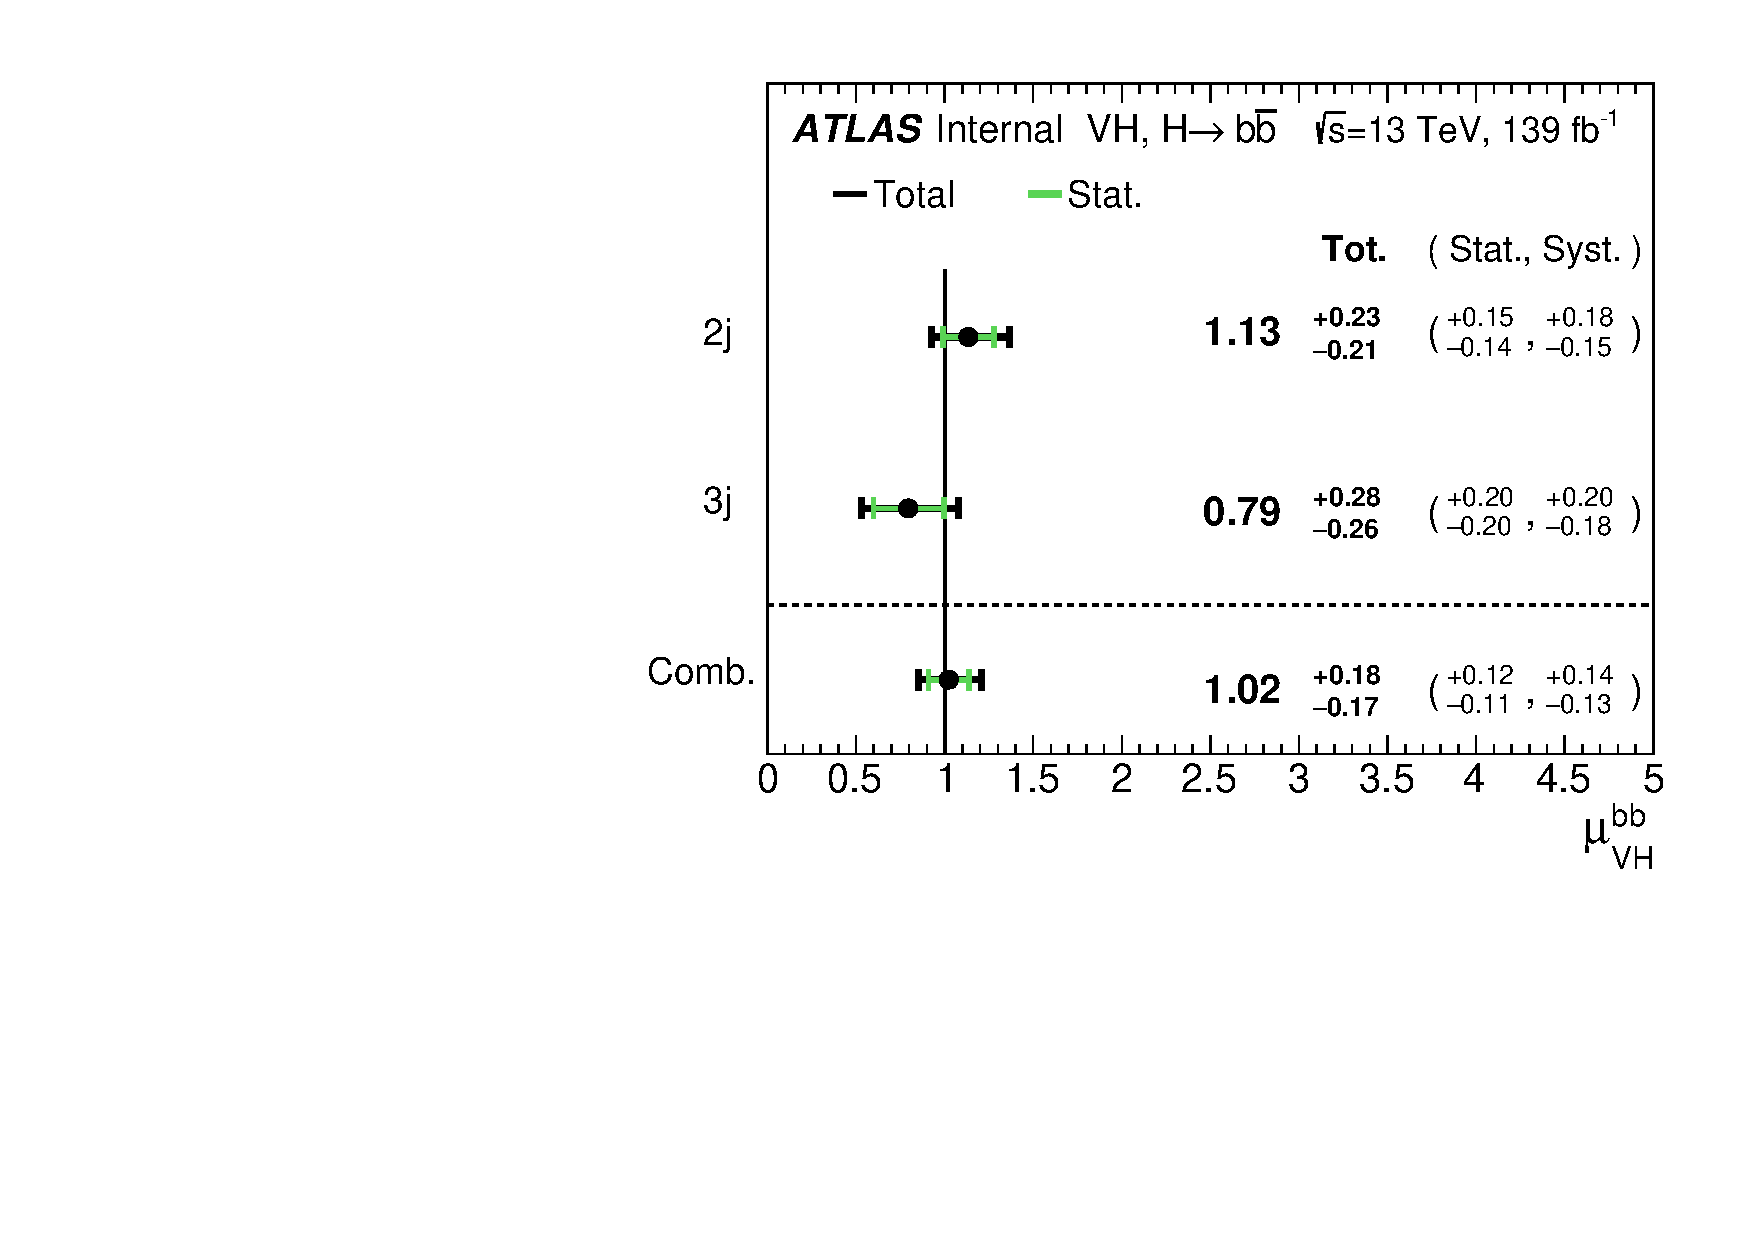
\includegraphics[width=0.47\linewidth]{final_fit_mva/results/Plot_mu_1_DecorrPOI_J_VH.pdf}
	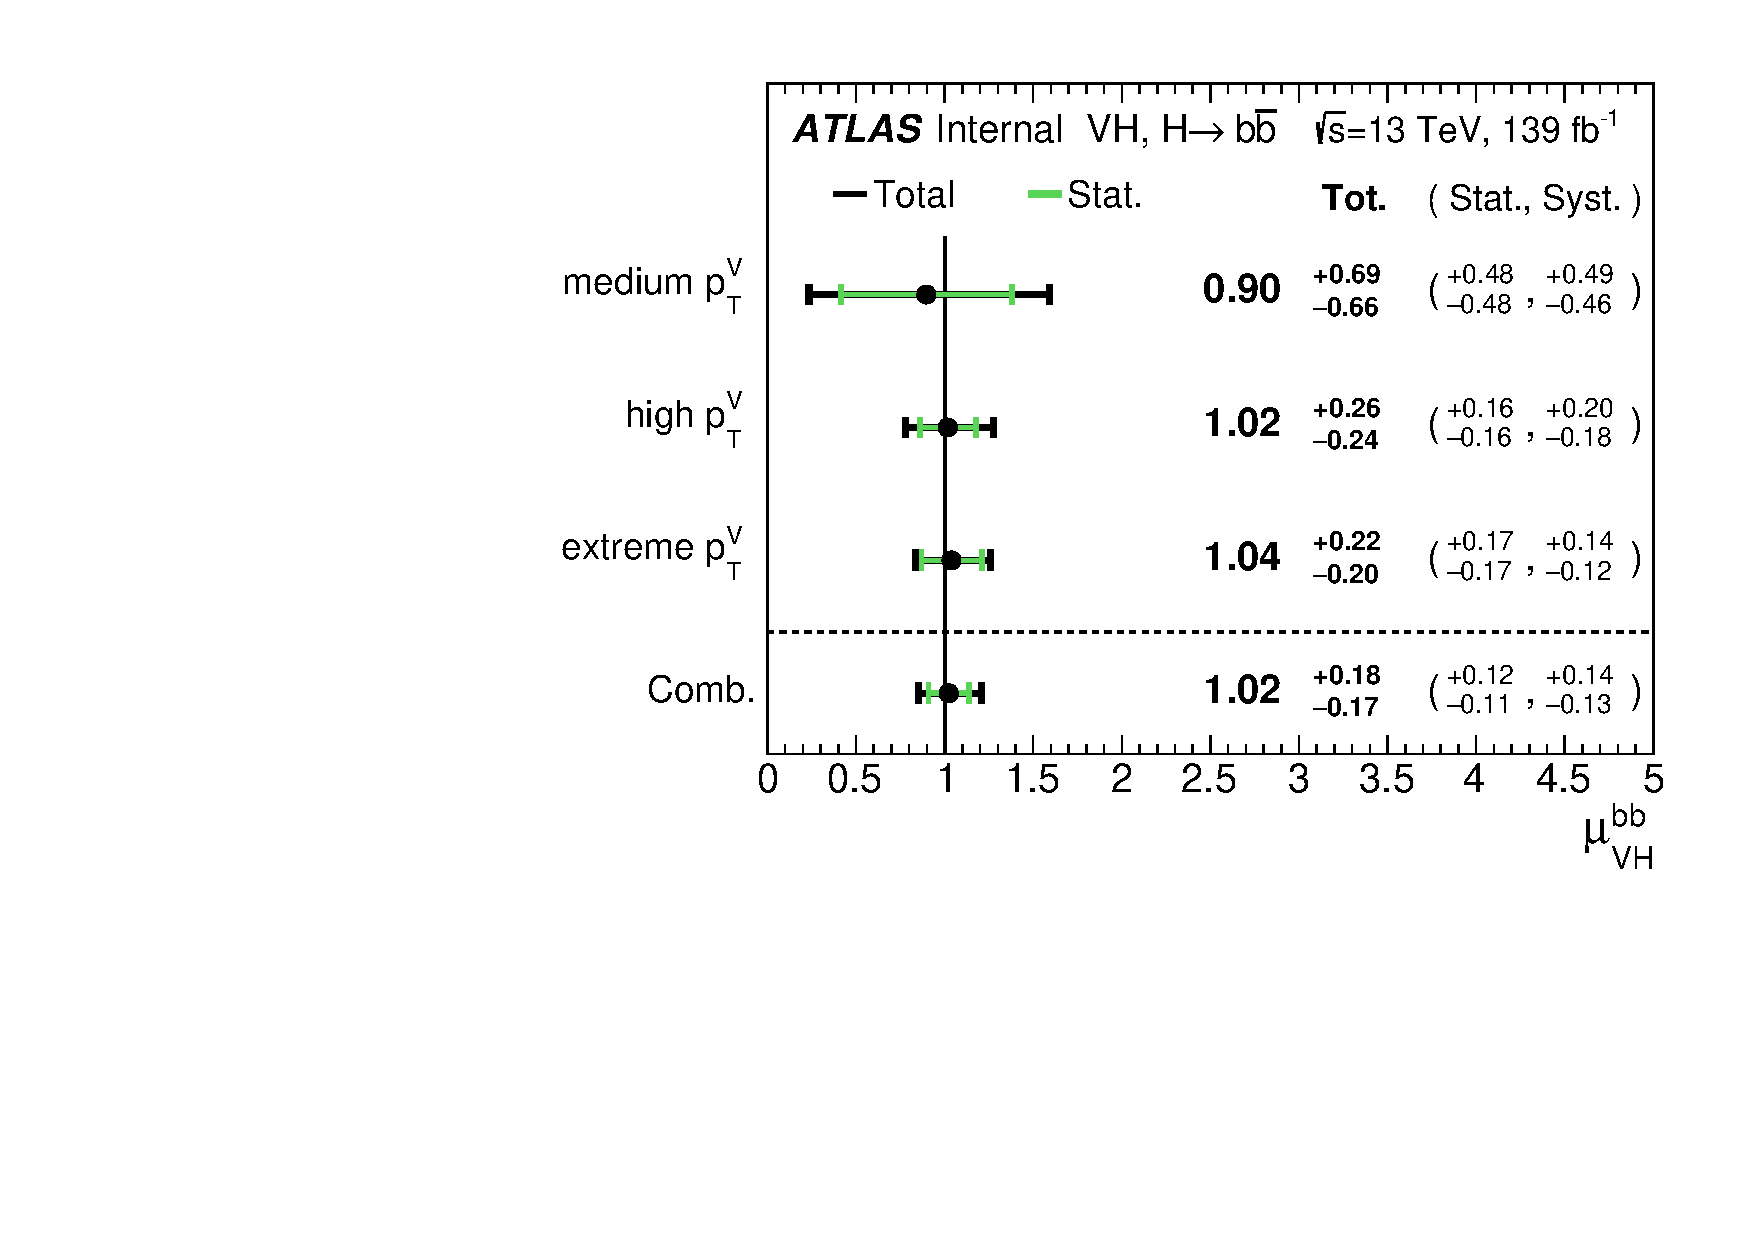
\includegraphics[width=0.47\linewidth]{final_fit_mva/results/Plot_mu_0_DecorrBMin_VH.pdf}
	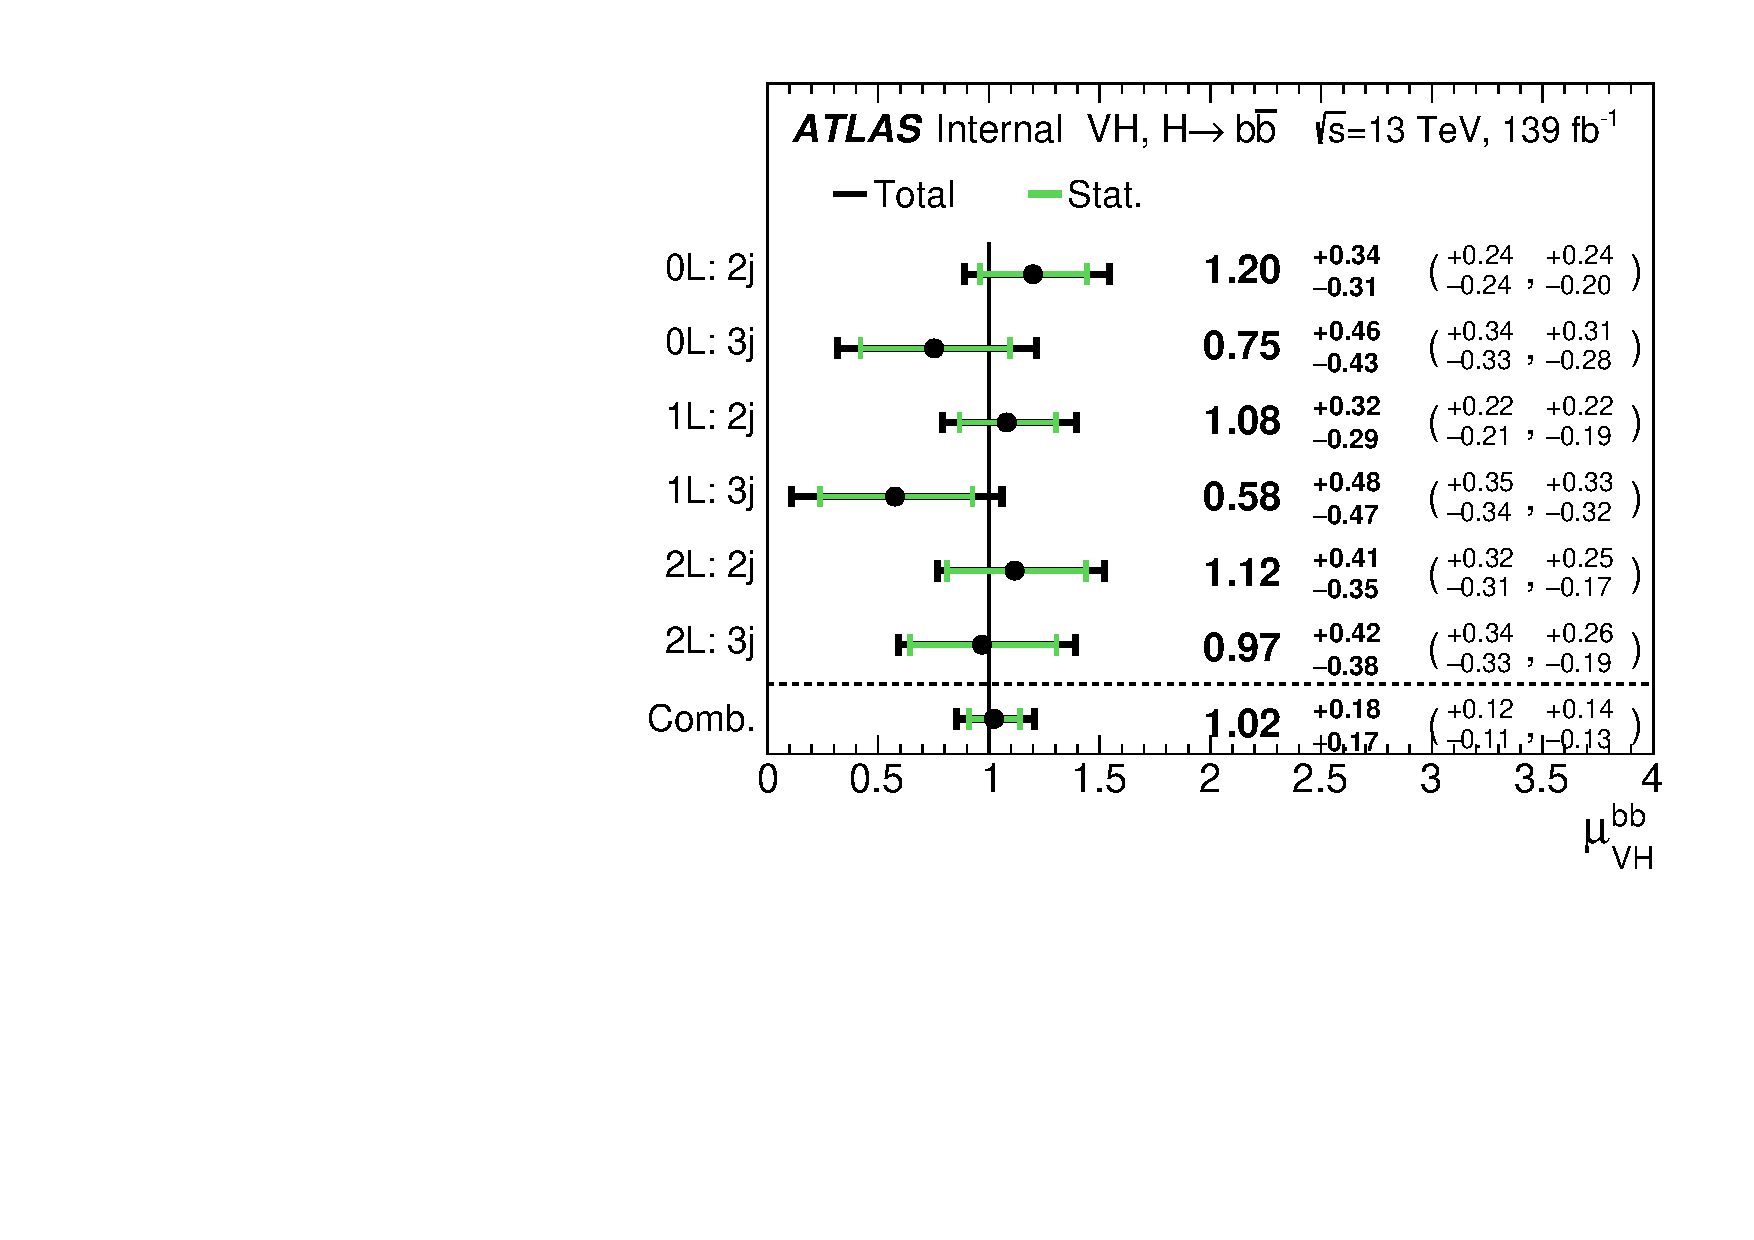
\includegraphics[width=0.47\linewidth]{final_fit_mva/results/Plot_mu_15_DecorrPOI_J_L_VH.pdf}
	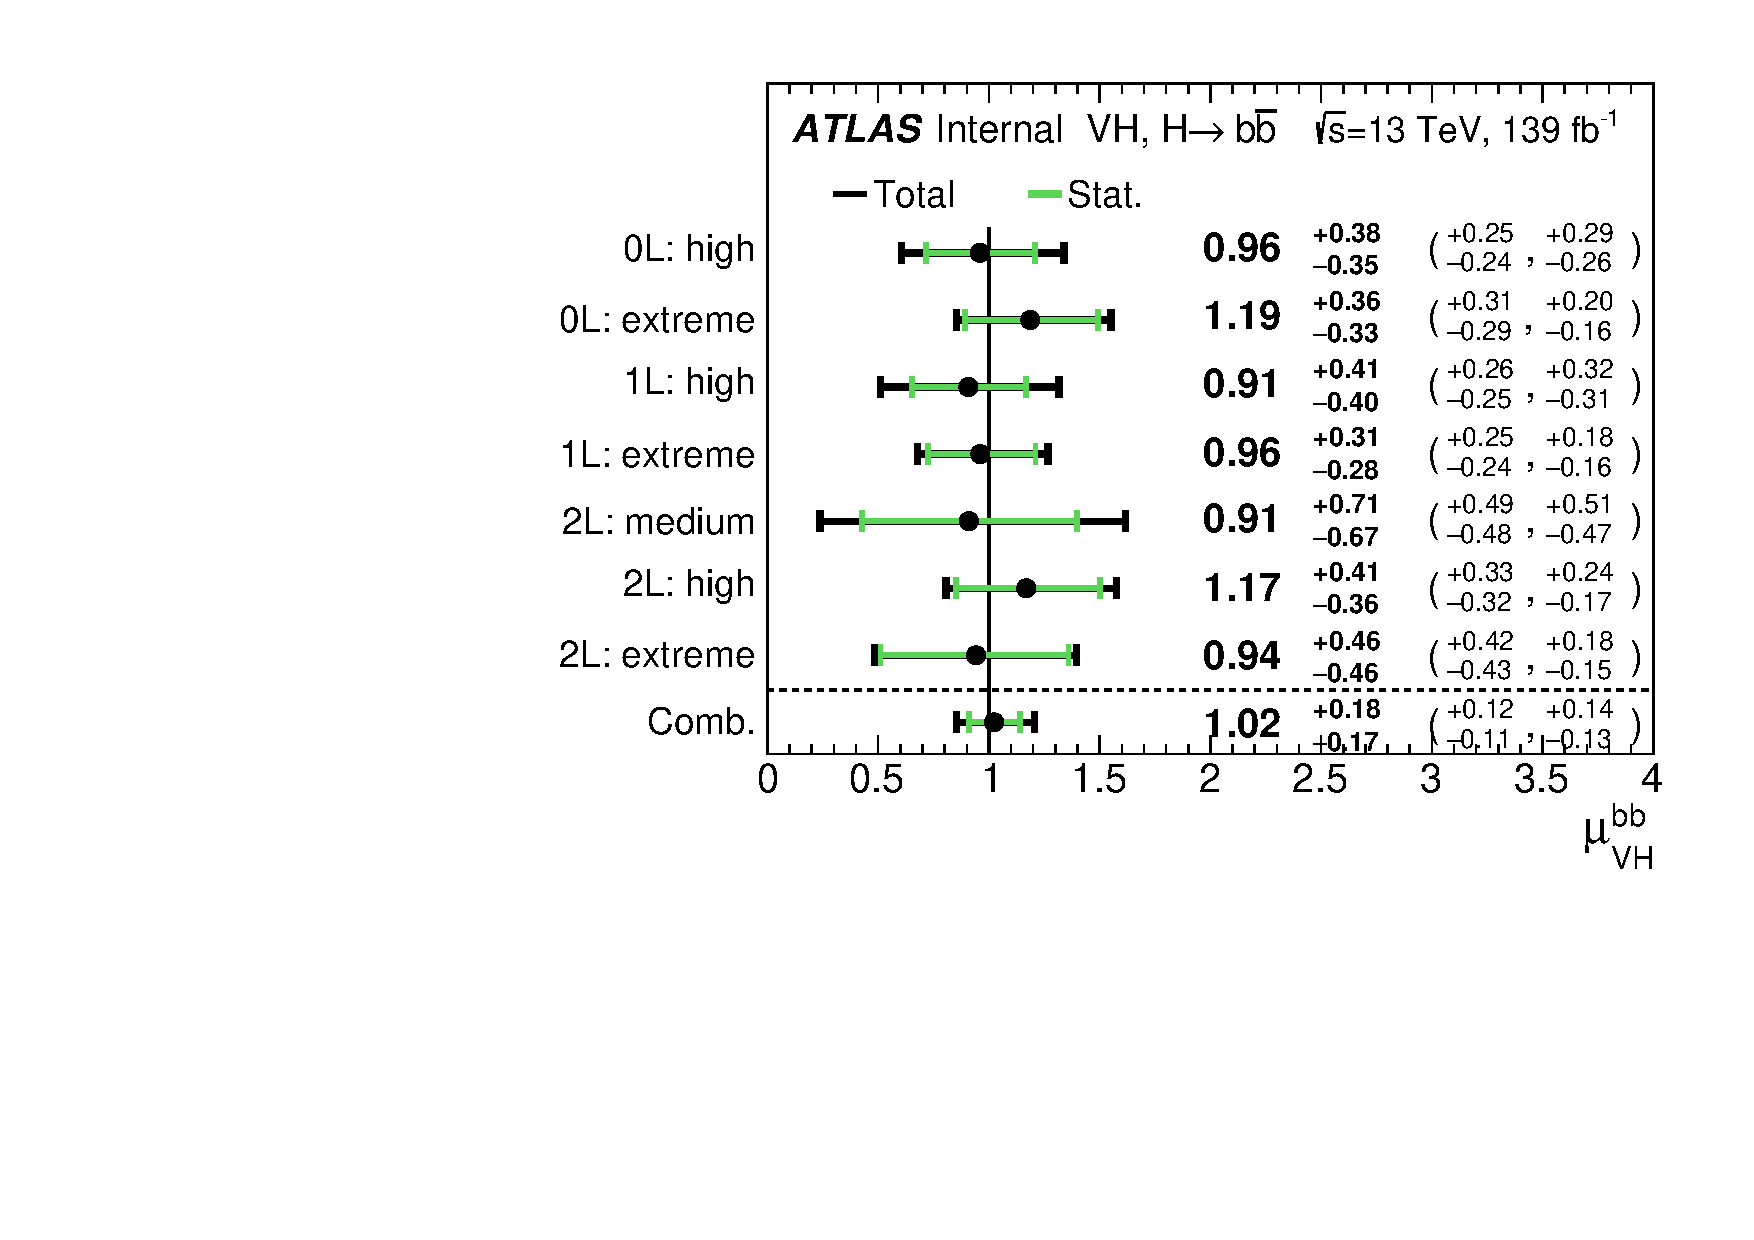
\includegraphics[width=0.47\linewidth]{final_fit_mva/results/Plot_mu_15_DecorrPOI_BMin_L_VH.pdf}
  \caption{caption}
  % Best values of the signal strength $\mu_{\VH}^{b\bar{b}}$ uncorrelated
  % (multi-$\mu$) between $N($jet$)$ regions (top left), \pTV regions (top right),
  % $N($jet$)$ regions and lepton channels (bottom left), \pTV regions and lepton
  % channels (bottom right) and their combination in the combined unconditional
  % fit to the Run 2 data. The (black) total observed uncertainty is quoted
  % together with its decomposition in the (green) statistical component, and
  % systematic component. In this plot the uncertainty due to background scale
  % factors is included in the statistical component.
\label{fig:channels-mus-uncorr}
\end{figure}